\section{Crypto Recap}
\subsection{Objectives:}
\begin{itemize}
  \item{\textbf{Confidentiality}}
  \item{\textbf{Integrity}}
  \item{\textbf{Authenticity}}
  \item{\textbf{Availability}}
  \item{Authorization}
  \item{Non-Repudiation, Accountability}
  \item{Freshness}
  \item{Anonymity, Unlinkability}
  \item{Intervenability, Contro}
  \item{Transparency}
\end{itemize}

\subsection{Confidentiality-Encryption}
\subsubsection{Symmetric Ciphers}
\begin{itemize}
  \item Secret key for en- and decryption
  \item Much more efficient
  \item \textbf{Block cipher: }encryps a plaintext block of fixed len e.g.: \textit{Advanced Encryption Standard (AES)}
  \item \textbf{Stream cipher: }encrypts a bitstream e.g.:\textit{ChaCha20}
\end{itemize}

\subsubsection{Asymmetric Ciphers}
\begin{itemize}
  \item Public key for encryption
  \item Private key for decryption
  \item Ex.: RSA-based encryption
\end{itemize}

\subsection{Integrity, Authenticity-Signatures, MACs}
\subsubsection{MACs}
\begin{itemize}
  \item Symmetric cryptography
  \item Protects data integrity \& authenticity
  \item Ex.: Hash-based MAC
\end{itemize}

\subsubsection{Digital Signatures}
\begin{itemize}
  \item Asymmetric cryptography
    \begin{itemize}
      \item{\textbf{Signing with} private key}
    \end{itemize}
  \item{Protects data integrity \& authenticity}
  \item{Provices non-repudation}
\end{itemize}

\subsection{Block Cipher Modes of Operation}
\subsubsection{Electronic Code Book (ECB)}
\begin{itemize}
  \item{Each plaintext block is encrypted seperatly}
  \item{Inherintly insecure! -> Smae block = Same cipher}
\end{itemize}

\subsubsection{Cipher Block Chainning (CBC)}
\begin{itemize}
  \item Plaintext is chained to previous ciphertext by XOR and encrypted afterwards
  \item Difficult to apply securely -> implementations often vulnerable
\end{itemize}

\subsubsection{Galois Counter Mode (GCM)}
\begin{center}
  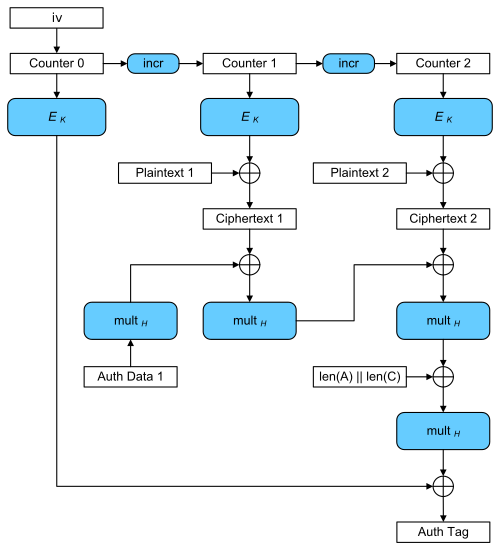
\includegraphics[width=0.5\columnwidth]{Resources/GCM-Galois_Counter_Mode_with_IV.svg.png}
\end{center}

\section{Tranport Layer Security (TLS)}
\subsection{TLS handshake protocol}
\begin{itemize}
  \item Parameter Negotiation
  \item Key exchange
  \item Authentication
\end{itemize}
\subsection{TLS record protocol}
\begin{itemize}
  \item Protection of integrity, authenticiy and confidentiality
  \item \textbf{Symmetric Cryptography:} e.g., block cipher, usually AES
\end{itemize}
